% ===========================================================================
\section{Introduction}
\label{sec:intro}

Language models now grade other language models. Evaluation leaderboards,
reward models and automated monitors all use an LLM judge, and the judge and
the judged usually come from the same small pool of models. A judge that
favours its own outputs is a known source of error
\citep{panickssery2024selfpreference, wataoka2024perplexity, ye2025justice},
and the standard defence is to remove the author's name before judging. That
defence assumes the judge cannot tell who wrote a text from the text itself.

\begin{figure*}[t]
  \centering
  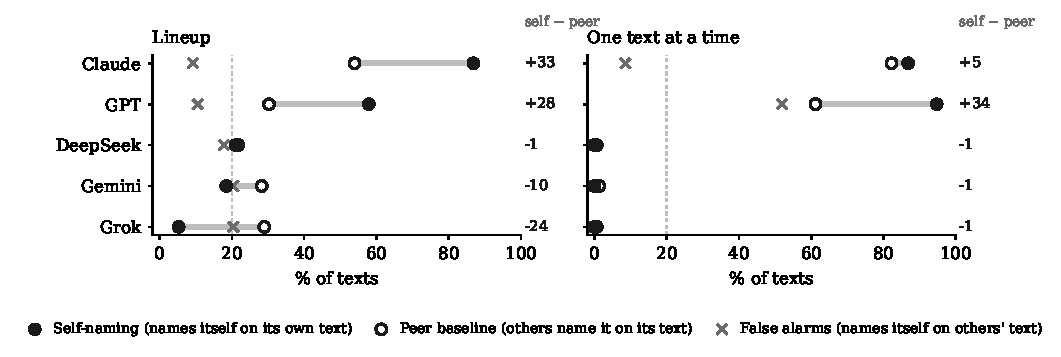
\includegraphics[width=\textwidth]{figures/lead.pdf}
  \caption{A self-naming rate (filled) means little on its own. Read it
  against the peer baseline (open: how often the other four judges name this
  judge on its text) and the false-alarm rate ($\times$: how often the judge
  names itself on text it did not write). Frontier panel, 38 texts per judge;
  the right-hand numbers are the self-advantage in points; dashed line, the
  20\% chance floor. In the lineup Claude and GPT beat their peers, Grok
  trails them. One text at a time, three judges never name themselves, and
  Claude's rate is matched by its peers.}
  \label{fig:lead}
\end{figure*}

Whether it can is usually measured with one number: how often a judge names
itself as the author of its own text, compared with chance. We argue that
this number, which we call the \emph{self-naming rate}, cannot answer the
question. A judge that names itself on 87\% of its own responses may
recognise its writing, or it may write text that \emph{anyone} can
attribute, or it may simply say ``me'' to everything. Separating the three
takes two more numbers from the same experiment (Figure~\ref{fig:lead}): how
often the judge names itself on text it did \emph{not} write (its
false-alarm rate), and how often the \emph{other} judges name it on its text
(its peer baseline). A judge recognises itself only if it beats that peer
baseline, a positive \emph{self-advantage}, and names itself more often on
its own text than on others', which we call \emph{discrimination}.

\begin{table}[t]
\centering\small
\setlength\tabcolsep{3pt}
\begin{tabular}{lll}
\toprule
Setting & Standard test & Our test \\
\midrule
Frontier, chat app, lineup & GPT, Claude & GPT, Claude \\
Frontier, chat app, single & GPT, Claude & GPT \\
Frontier, API, lineup & Claude, Grok & -- \\
Frontier, API, single & GPT, Claude & -- \\
Open-weight, lineup & Qwen & -- \\
Open-weight, single & Qwen, Llama, Phi & -- \\
Open-weight, yes/no & Llama, Mistral & -- \\
\midrule
Judge-settings flagged & 14 of 32 & 3 of 32 \\
\bottomrule
\end{tabular}
\caption{Which judges ``recognise themselves''. Standard test: the judge names itself on its own text more often than chance (Holm-corrected binomial test; for yes/no, says yes to its own text more than half the time). Our test: it beats its peers on its own text \emph{and} names itself more on its own text than on others' (both Holm-corrected permutation tests; for yes/no, AUC above 0.5). Nine judges, three corpora, three formats.}
\label{tab:verdicts}
\end{table}


We apply both tests to nine judges on three corpora. Five frontier models
(GPT-5.5, Claude Opus 4.7, Gemini 3.5 Flash, Grok 4.3 and DeepSeek)
attribute 190 texts they wrote in their chat apps for 38 prose prompts, and
600 texts they wrote through the API for 120 prompts in four genres
(argumentative prose, code, short answers and worked math). Four
open-weight models from four labs attribute \OWNResponses{} texts they wrote
for the same 120 prompts; their weights also let us read each judge's
likelihood of every text and rule out vendor watermarks. Judges name authors
in a lineup and one text at a time, and the open-weight judges also answer
``did you write this?'', in a fresh context or with their own answer to the
task in the conversation.

Three findings follow.
\begin{enumerate}
\item \textbf{The standard test is mostly wrong.} Of \SVPCells{}
judge--settings, the self-naming rate exceeds chance in \SVPStd{}; only
\SVPProper{} pass our test (Table~\ref{tab:verdicts}). The \SVPFalse{} false
positives (\SVPFalsePct{}) are judges that name themselves on much of what
they read: one text at a time GPT names itself on \FXGPTSingleNamesSelf{} of
all texts and Llama on \OWLlamaSingleNamesSelf{}, and asked ``did you write
this?'' Mistral says yes to \OWMistralBinaryFA{} of texts it did not write.
The standard test never missed a judge ours found.
\item \textbf{Real self-recognition is rare and does not travel.} Only Claude
and GPT pass, and only on the chat-app texts, where Claude's self-advantage
is \ClaudeAdvLineup{} points \ClaudeAdvLineupCI{} and GPT's \GPTAdvLineup{}.
On the 600 API texts no judge beats its peers, who name Claude's text almost
as readily as Claude does (\FXClaudeLineupPeer{} against
\FXClaudeLineupSelf{}). What holds across corpora is Claude's
discrimination: it names itself on \FXClaudeLineupSelf{} of its own texts and
\FXClaudeLineupFA{} of others'.
\item \textbf{Judges have the signal and do not use it.} A stylometric
classifier attributes the frontier texts at \EngineAAcc{} and the open-weight
texts at \OWClfPooled{}, and each open-weight judge's own likelihood picks
out its own text on \OWLikCondAccMin{} of prompts; yet what a judge claims as
its own does not follow its likelihood in any format, and none of the 1,900
reasons the frontier judges gave refers to the judge itself.
\end{enumerate}

The audit we propose needs no extra data, only the judgments a lineup
already produces (Section~\ref{sec:recs}): report a self-naming rate with its
false-alarm rate and peer baseline, test discrimination, never measure
recognition one text at a time, and measure each judge on the kind of text
it will judge. The stakes go beyond leaderboards: a monitor that reviews the
output of a copy of itself is only as independent as its inability to
recognise that output \citep{khullar2026selfattribution}.
